\section{Cloud Architektur}

Bei den Cloud Architekturen gibt es genau 3 verschiedene Rollen:
\begin{enumerate}
	\item \textbf{Provider:} bietet Cloud Produkte/Lösungen an
	\item \textbf{Konsumenten:} konsumieren Cloudlösungen
	\item \textbf{Klient:} nehmen Cloudlösungen (Anwendungen/Daten) in Anspruch
\end{enumerate}

\subsection{Konzeptuelle Sichtweise}

In diesem Abschnitt werden die Architekturen der einzelnen Kategorien von Cloudlösungen beschrieben.

\subsubsection{Konsumenten Sichtweise}

Wie in \textbf{Abbildung \ref{ConsumerView}} zu sehen, werden Ressourcen in Form von Clustersystemen vom Provider zur Verfügung gestellt.
Einzelne Klienten können über eine Netzwerkverbindung auf diese Ressourcen zeitgleich zugreifen. Der Provider kann außerdem den Pool
von Hardware Ressourcen verwalten, d.h. einzelne Hardware kann stillgelegt und ersetzt werden. Die Klienten werden nach dem stilllegen
auf andere Hardware Ressourcen weitergeleitet.
\begin{figure}[H]
    \centering
	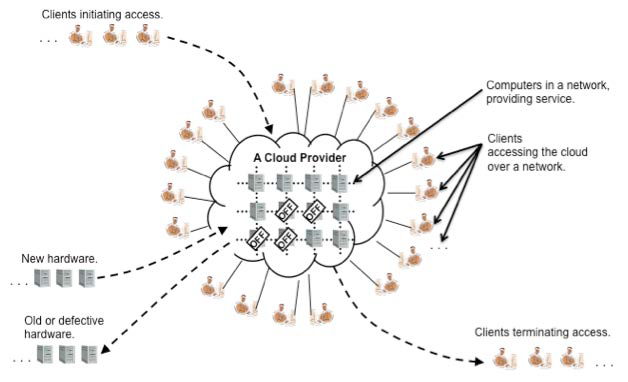
\includegraphics[width=0.4\textwidth]{Images/ConsumerView}
	\caption{Konsumenten Sichtweise \cite{Badger}}
	\label{ConsumerView}
\end{figure}

Alle Kategorien von Cloud-Computing können sogenannte Sicherheitsperimeter verwenden. Diese Regeln den Zugriff auf die Ressource.
In unseren Beispielen kann ein Klient, der sich außerhalb des Sicherheitsperimeter befindet, nur durch einen \glqq boundary controller\grqq
Zugriff zum Netzwerk erlangen.

\subsubsection{Lokale Private Cloud}

Wie in \textbf{Abbildung \ref{PrivateCloud}} zu sehen, befindet sich eine Private Cloud innerhalb der Organisation.
Klienten, die sich innerhalb des Sicherheitsperimeters befinden, können sich mit der Privaten Cloud verbinden. 
Klienten von außerhalb, können eine Verbindung durch den \glqq boundary controller\grqq aufbauen. Dieser Sicherheitsperimeter ist in diesem
Fall optional und wird von dem Konsumenten verwaltet.

\begin{figure}[H]
    \centering
	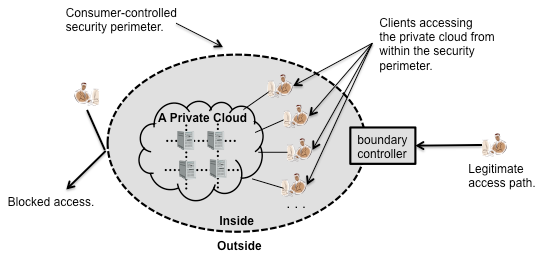
\includegraphics[width=0.4\textwidth]{Images/On-sitePrivateCloud}
	\caption{Private Cloud \cite{Badger}}
	\label{PrivateCloud}
\end{figure}

Die Verwaltung der Cloud wird vom Konsumenten übernommen. Dieser muss die Cloud so einstellen, dass die Arbeitslast zwischen verschiedenen
Maschinen verteilt werden kann, um die Ressourcen optimal nutzen zu können. Außerdem sollten redundante Kopien der Daten auf verschiedenen Maschinen 
gespeichert werden. Dies hat den Vorteil, dass bei einem Serverausfall der Klient auf eine andere Maschine weitergeleitet werden kann.
Außerdem muss der Konsument sicherstellen, dass wichtige Daten wie z.B. Lohnabrechnungen nicht von allen Klienten zugegriffen werden können,
da verschiedenen Daten auf einer Maschine verarbeitet werden können. Der Nachteil von Privaten Clouds ist, dass es hohe Anschaffungskosten, wie z.B. 
das Anschaffen von neuen Daten Zentren, gibt. Außerdem müssen bei z.B. steigenden Zugriffszahlen, neue Hardware vom Konsumenten bereitgestellt werden. 
Dies verringert Flexibilität des Konsumenten.

\subsubsection{Ausgelagerte Private Cloud}

Bei der ausgelagerten Privaten Cloud, wird die Cloud zu einem Provider verlagert. Dieser separiert das Organisationsnetzwerk
von seinem \glqq öffentlichen\grqq Netzwerk, wie in \textbf{Abbildung \ref{OutSourcedPrivateCloud}} zu sehen ist. Das Netzwerk wird vom Provider
durch einen Sicherheitsperimeter geschützt. Der Provider muss dabei sicherstellen, dass die Sicherheitsanforderungen des Konsumenten erfüllt werden. 
Der Konsument kann ebenfalls einen Sicherheitsperimeter in seiner Organisation installieren, um den Zugriff zur Cloud zu regeln.
Die beiden Perimeter werden dann durch einen Kommunikationskanal verbunden und Klienten können dann nur über diesen Kanal auf Daten der Cloud zugreifen.

\begin{figure}[H]
    \centering
	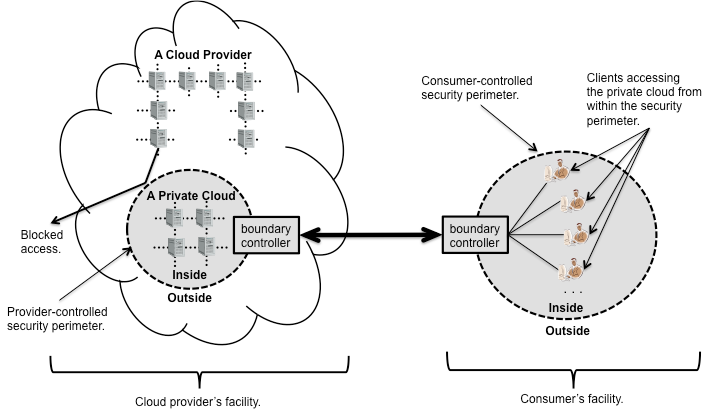
\includegraphics[width=0.4\textwidth]{Images/OutSourcedPrivateCloud}
	\caption{Ausgelagerte Private Cloud \cite{Badger}}
	\label{OutSourcedPrivateCloud}
\end{figure}

Der Konsument ist in diesem Fall von der Netzwerkverfügbarkeit und -geschwindigkeit des Providers abhängig, kann die Geschwindigkeit aber durch Sondertarife erhöhen.
Der Provider muss außerdem sicherstellen, dass die Arbeitslast auf den verschiedenen Maschinen innerhalb des Perimeters verteilt wird und sich die Daten 
nicht mit den Daten von anderen Organisationen, außerhalb des Perimeters, vermischen.
Der Vorteil dieser Architektur ist es, dass der Konsument keine eigenen Ressourcen mehr anschaffen muss und diese beim Provider mieten kann.
Eine Erhöhung der verfügbaren Ressourcen kann jedoch vom Provider nur manuell geschehen, sofern dieser über genug Ressourcen verfügt. 

\subsubsection{Lokale Community Cloud}

Bei der Lokalen Community Cloud teilen mehrere Organisationen ihre Ressourcen und Daten. Alle Organisation stellen und/oder konsumieren Cloud Services.
Dabei muss mindestens eine Organisation solche Services zur Verfügung stellen. Somit ist mindestens eine Organisation, sowohl Provider als auch Konsument.
Sollte jede Organisation einen Sicherheitsperimeter installieren, werden die einzelnen Organisationen durch Kommunikationskanäle zwischen den \glqq boundary controller\grqq verbunden.
Organisationen können außerdem einen weiteren Sicherheitsperimeter einrichten, um die lokalen Cloud Ressourcen von den lokalen Ressourcen zu trennen.

\begin{figure}[H]
    \centering
	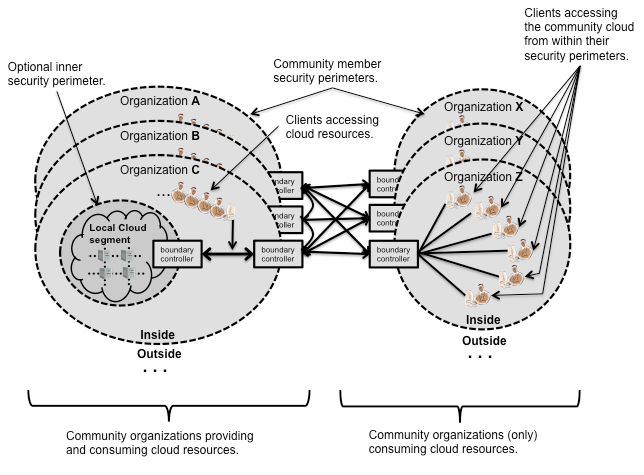
\includegraphics[width=0.4\textwidth]{Images/On-siteCommunityCloud}
	\caption{Lokale Community Cloud \cite{Badger}}
	\label{On-siteCommunityCloud}
\end{figure}

Für die Verwendung der lokalen Community Cloud wird eine komplexe Sicherheitsauthentifizierung benötigt. Jede Organisation der Community muss einen Zugriff bieten und erhalten.
Außerdem müssen die Kommunikationskanäle geschützt und bei der Verwendung des öffentliche Internet Kryptographie verwenden werden. Die einzelnen Kommunikationskanäle zwischen den Teilnehmern 
können verschiedene Level der Performance, Sicherheit und Zuverlässigkeit bereitstellen, abhängig von den Ansprüchen der Teilnehmenden Organisationen. Die Sicherheit der einzelnen Clouds hängt 
hierbei von den den Sicherheitsperimeter der einzelnen Organisationen ab. Ein großer Nachteil dieser Methode sind die hohen Kosten der einzelnen Provider, die Ressourcen 
anschaffen und Services konfigurieren müssen. Die Konsumenten hingegen zahlen nur die Mietkosten der für die Verwendungen der einzelnen Clouds. Ein weiterer Nachteil ist, dass 
die Ressourcen lokal bereitgestellt werden und somit limitiert sind. Wodurch die Flexibilität der einzelnen Organisationen sinkt.

\subsubsection{Ausgelagerte Community Cloud}

Bei der Ausgelagerten Community Cloud verhält es sich ähnlich zu der Ausgelagerten Privaten Cloud, wie in \textbf{Abbildung \ref{OutSourcedCommunityCloud}} zu sehen ist.
Um die Serverseitige Verantwortung kümmert sich hier der Provider, der ein Sicherheitsperimeter installiert und verwaltet. Dabei sorgt der Provider dafür, dass sich 
die Community Ressourcen und die Cloud Provider Ressourcen, die sich außerhalb des Perimeters befinden, nicht vermischen. Ein wesentlicher Unterschied zur Ausgelagerten Privaten Cloud
besteht darin, dass der Cloud Provider möglicherweise eine Freigaberichtlinie zwischen den teilnehmenden Unternehmen der Community Cloud durchsetzen muss. 
Um den Organisationen der Community Konsumenten eine Verbindung zur Cloud zu ermöglichen, müssen sichere Kommunikationskanäle zwischen den einzelnen Organisationen und 
dem Provider installiert werden. 

\begin{figure}[H]
    \centering
	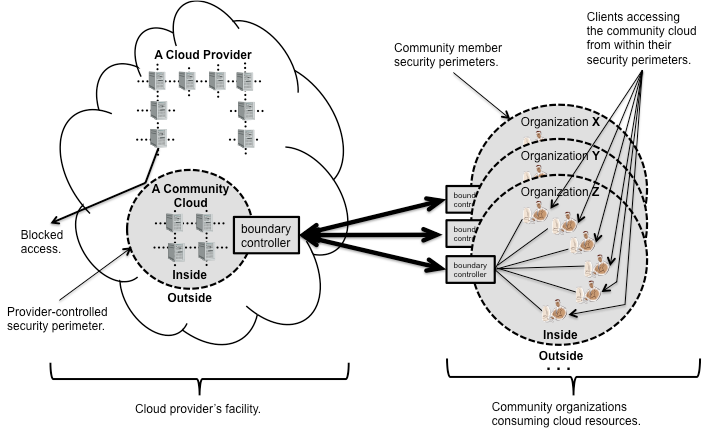
\includegraphics[width=0.4\textwidth]{Images/OutSourcedCommunityCloud}
	\caption{Ausgelagerte Community Cloud \cite{Badger}}
	\label{OutSourcedCommunityCloud}
\end{figure}

\subsubsection{Public Cloud}

Die Public Cloud, die in \textbf{Abbildung \ref{PublicCloud}} zu sehen ist, verhält sich recht ähnlich zu \textbf{Abbildung \ref{ConsumerView}}.
Außer das der Konsument einen eigenen Sicherheitsperimeter installiert, um den Zugriff zur Cloud zu regeln.

 
\begin{figure}[H]
    \centering
	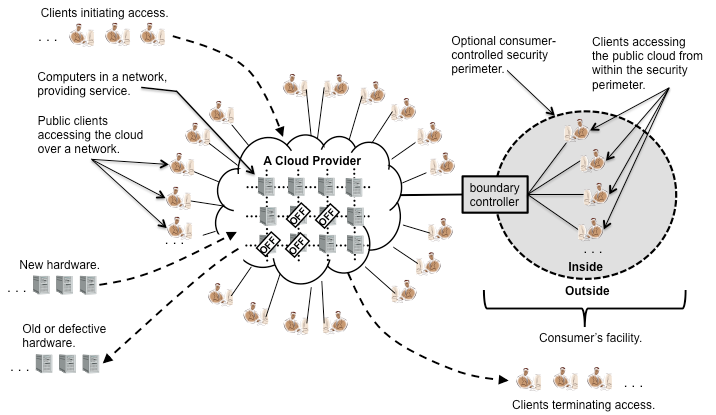
\includegraphics[width=0.4\textwidth]{Images/PublicCloud}
	\caption{Public Cloud \cite{Badger}}
	\label{PublicCloud}
\end{figure}

In diesem Szenario verbindet sich der Konsument über das öffentliche Internet, sodass die Verbindungsqualität und -zuverlässigkeit zur Cloud
von dem Internet Provider, dem DNS Server und der Router Infrastruktur abhängt. Die Arbeitslast oder Ressourcen eines Konsumenten können zu jeder Zeit
vom Provider migriert werden. Ein großer Vorteil der Public Cloud ist die Kosteneffizient, da Datenzentren an Standorten verwendet werden können, die für den Konsumenten am günstigen sind.
Ein Beispiel dafür wäre, das die Arbeitslast eines Deutschen Unternehmens in einem Deutschen Datenzentrum verarbeitet und somit die Performance verbessert wird (geringe Übertragungswege).
Dies wird aber meist nicht von Provider versichert. Die Arbeitslast kann an verschiedenen Standorten (Europa, USA, China usw.) verarbeitet werden, außer der Provider bietet eine
Standortbeschränkung an. Ein großes Problem der Public Cloud ist es, dass eine Maschine die Daten von mehreren Konsumenten verarbeiten kann und somit ein Sicherheitsrisiko entstehen kann.
Außerdem haben die Konsumenten keine Möglichkeit die Einsicht ihrer Daten zu überwachen oder eine Authentifizierung für ihre Daten einzurichten. Da große Anbieter meist eine Monitoring für die
Daten durchführen, um die Tatsächliche Datennutzung zu ermitteln und den Konsumenten diese dann in Rechnung zu stellen, ist diese Methode nicht für sensible oder wichtige Daten geeignet.
Außerdem kann der Konsument nie sicher sein, ob sein Daten auch gelöscht werden, wenn er den Vertrag kündigt. 
Ein großer Vorteil der Public Cloud ist die Uneingeschränktheit in Hinsicht des Standortes und der Größe. D.h. die Größe der zur Verfügung gestellten Ressourcen lässt sich 
meist \glqq uneingeschränkt\grqq erhöhen oder vermindern.

Bekannte Public Cloud Provider sind Amazon Web Services (AWS) und Microsoft Azure. 

% \subsubsection{Hybrid Cloud}
% Eine Hybrid Cloud besteht aus mindestens zwei oder mehreren Privaten, Community oder Public Clouds.
% \begin{figure}[H]
%     \centering
% 	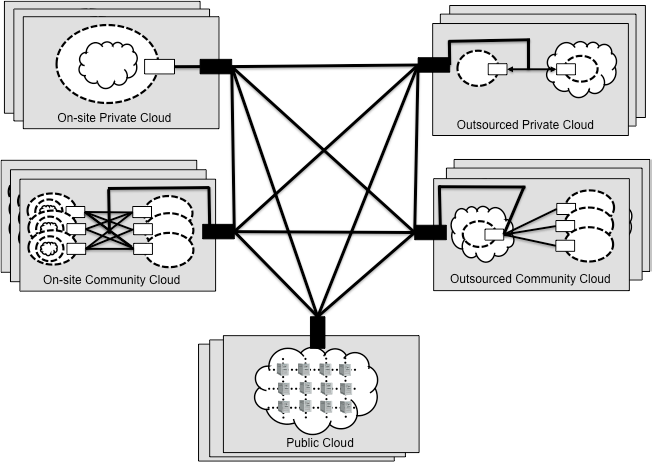
\includegraphics[width=0.5\textwidth]{Images/HybridCloud}
% 	\caption{Hybrid Cloud \cite{Badger}}
% 	\label{HybridCloud}
% \end{figure}

\subsection{Architekturen der Dienstmodelle}

In diesem Abschnitt werden die Architekturen der drei Dienstmodelle SaaS, PaaS, IaaS beschrieben.

\subsubsection{SaaS}\label{SaaS Architektur}

\begin{figure}[H]
    \centering
	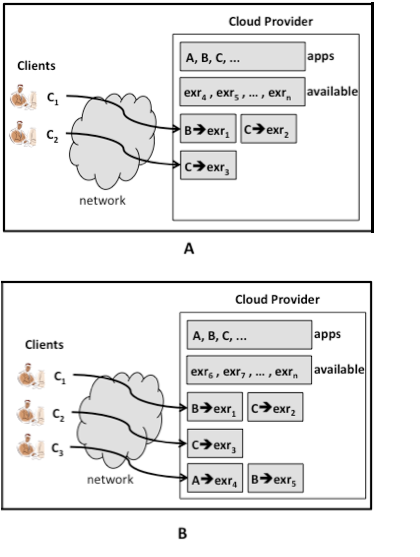
\includegraphics[width=0.4\textwidth, height=8cm]{Images/SaaSInteraction}
	\caption{SaaS Interaktion \cite{Badger}}
	\label{SaaSInteraction}
\end{figure}
Wie bereits in Abschnitt \ref{IaaS} beschrieben, stellt der Provider den Klienten Anwendungen (\glqq Apps\grqq) zu Verfügung.
Diese Anwendungen können dann über das öffentliche Internet (Webseiten) aufgerufen werden.
Wie in \textbf{Abbildung \ref{SaaSInteraction}.A} zu sehen ist, kann ein Provider mehrere Apps anbieten und ausführen.
Er hat dabei eine gewisse Anzahl an \glqq Execution Ressources\grqq (exr) zur Verfügung. 
Dabei wird den Klienten bei jedem starten einer Anwendung eine exr zugewiesen. Sollten neue Klienten hinzukommen, werden ihm verbleibende Ressourcen (exr) zugewiesen. 

\begin{figure}[H]
    \centering
	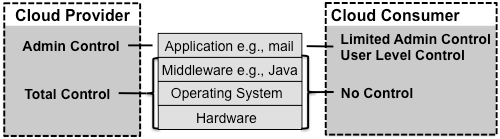
\includegraphics[width=0.45\textwidth]{Images/SaaSControl}
	\caption{SaaS Kontrollverteilung \cite{Badger}}
	\label{SaaSControl}
\end{figure}

\textbf{Abbildung \ref{SaaSControl}} zeigt, wie die Kontroll- und Managementverantwortung zwischen den Provider und den Konsumenten verteilt wird.
Bei Software as a Service hat der Konsument nur die Kontrolle auf der Benutzerebene, d.h. dieser kann Benutzerverwalten wie z.B. Benutzer hinzufügen.
Der Provider hingegen verfügt die totale Kontrolle über alle Bereiche. Diese muss ist Verantwortlich für das Erstellen, konfigurieren und Verwalten der Anwendungen, 
sodass der Konsument diesen Service nutzen kann.
Bei der Middleware Schicht kann der Provider sowohl über die Software Bibliotheken, als auch Datenbankenservices entscheiden, der Konsument hat darauf keinen Einfluss.
Das selbe gilt bei der Wahl des Betriebssystems und der Hardware, bei der der Konsument keinen Einfluss hat.

\subsubsection*{Vorteile von SaaS}

Im Vergleich zu traditionellen Computing- und Softwareverteilungslösungen bieten SaaS-Clouds Skalierbarkeit und verlagern zudem die Belastungen vom Konsumenten zum Provider.
Die Vorteile eines solchen Services sind, dass für öffentliche und ausgelagerten Szenarien, sich der Großteil der von einer Anwendung verwalteten Daten auf den Softwareverteilungslösungen
des Cloud-Providers befinden. Der Provider kann diese Daten dezentral und redundant speichern, sodass ein Verlust von Daten unwahrscheinlich wird. Außerdem bieten SaaS-Provider
ein professionelles Management System an, dass z.B. Compilance-Check (Datenschutz), Security-Scanning (Virenprüfung), Backup und Disaster Recovery unterstützt.

\subsubsection{Funktionsweise von SaaS}

Wie bereits erwähnt wird bei Starten einer Anwendung von einem Nutzer ein Prozess (exr) gestartet. Dabei haben die Provider meist eine statische oder eine dynamische
Lösung, um die Anwendung zu betreiben, wie \textbf{Abbildung \ref{SaaSM1}} zeigt.

\begin{figure}[H]
    \centering
	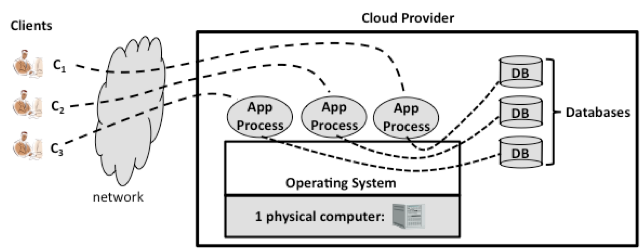
\includegraphics[width=0.5\textwidth]{Images/SaaSM1}
	\caption{Möglichkeit 1 \cite{Badger}}
	\label{SaaSM1}
\end{figure}

In diesem Szenario wird eine aktive Kopie der Anwendung für jeden Benutzer gestartet. Jede Anwendung betreibt dabei ein eigenes Datenbanksystem, indem die Daten der Benutzer gespeichert werden.
Somit besitzt jeder Klient eine eigene Kopie der Daten. Die einzelnen Kopien der Anwendung, der Datenbanksysteme und die Separierung der Benutzer wird durch das Betriebssystem ermöglicht.
Ein großer Nachteil dieses Szenarios ist es, dass hohe Kosten für das Betreiben und Synchronisieren der einzelnen Datenbanksysteme entstehen.

\begin{figure}[H]
    \centering
	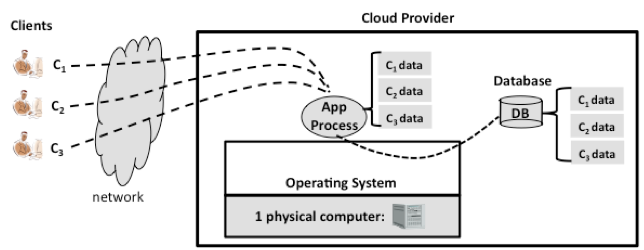
\includegraphics[width=0.5\textwidth]{Images/SaaSM2}
	\caption{Möglichkeit 2 \cite{Badger}}
	\label{SaaSM2}
\end{figure}

Beim statischen Szenario (\textbf{Abbildung \ref{SaaSM2}}) wird die Anwendung vom Provider so implementiert, sodass mehrere Klienten gleichzeitig daran arbeiten können und die Daten in nur einem Datenbanksystem gespeichert werden. 
Dies hat den Vorteil das die Kosten für den Provider gesenkt werden, da nur noch eine Anwendung betrieben wird.
Die Anwendung selbst, muss dafür aber die Daten mehrerer Klienten gleichzeitig verarbeiten und trotzdem sicherstellen, dass die Sicherheit der Daten gewährleistet ist.   

\subsubsection{Paas}
\todo{eventuell text anpassen}
Der Unterschied von Platform as a Service zu Software as a Service ist, dass Konsumenten die Möglichkeit haben, eigene Anwendungen bei dem Cloud Provider betreiben zu lassen.

\begin{figure}[H]
    \centering
	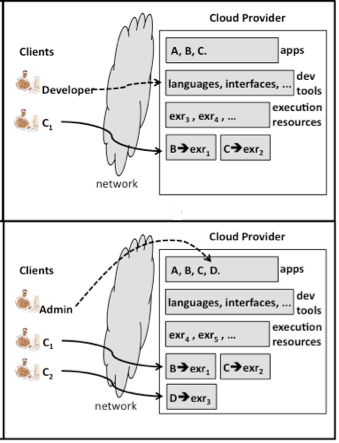
\includegraphics[width=0.4\textwidth]{Images/PaaSInteraction}
	\caption{PaaS Interaktion \cite{Badger}}
	\label{PaaSInteration}
\end{figure}

In der \textbf{Abbildung \ref{PaaSInteration}} wird gezeigt, wie sich die Interaktionen der einzelnen Nutzer verändern.
Der Klient kann weiterhin auf die Anwendungen (A, B, C) zugreifen. Beim Zugreifen wird hier ebenfalls ein neuer Prozess (exr) gestartet. Der Unterschied hier ist aber, dass
der Konsument für die Bereitstellung, Verwaltung, Aktualisierung der Anwendung zuständig ist. Der Provider bietet dem Konsumenten nur die Ressourcen um die Anwendung(en) zu betreiben.
Außerdem kann ein Provider ebenfalls Entwicklungswerkzeuge anbieten, die von den Entwicklern des Konsumenten verwendet werden können (z.B. eigene Datenbank).

\begin{figure}[H]
    \centering
	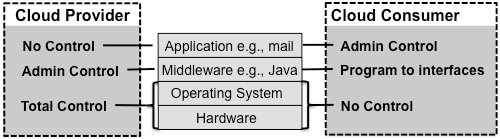
\includegraphics[width=0.45\textwidth]{Images/PaaSControl}
	\caption{PaaS Kontrollverteilung \cite{Badger}}
	\label{PaaSControl}
\end{figure}

Bei der Kontrolle der Schichten hat der Provider nur noch die Kontrolle über das Betriebssystem und die Hardware, wie die \textbf{Abbildung \ref{PaaSControl}} zeigt.
Sollte der Provider noch Entwicklungswerkzeuge anbieten so behält er die Administrative Kontrolle über diese Werkzeuge. Der Konsument hingegen hat im gegensatz zu SaaS,
die volle Kontrolle über die Anwendungen und falls er keine Entwicklungswerkzeuge nutzt, über die Middleware Schicht.

\subsubsection*{Vorteile von PaaS}

\subsubsection{IaaS}
aaa
\begin{figure}[H]
    \centering
	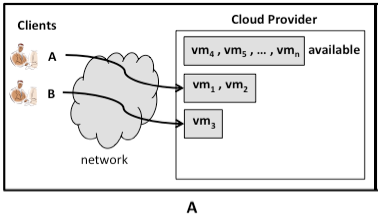
\includegraphics[width=0.5\textwidth]{Images/IaaSInteraction}
	\caption{IaaS Interaktion \cite{Badger}}
	\label{IaaSInteraction}
\end{figure}

aaa
\begin{figure}[H]
    \centering
	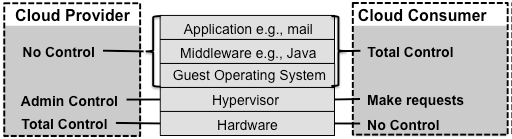
\includegraphics[width=0.5\textwidth]{Images/IaaSControl}
	\caption{IaaS Kontrollverteilung \cite{Badger}}
	\label{IaaSControl}
\end{figure}

\subsection{Logische Sichtweise}
aaaaaaaaa
\begin{figure}[H]
    \centering
	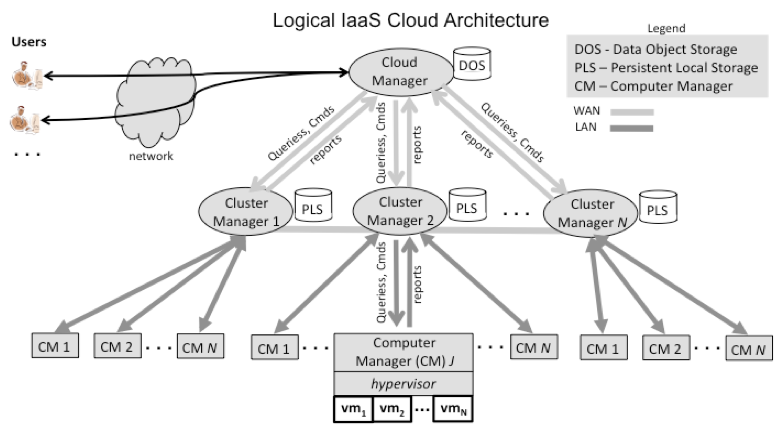
\includegraphics[width=0.5\textwidth]{Images/IaaSLogic}
	\caption{IaaS Logische Sichtweise (vgl. \cite{Badger})}
	\label{IaaSLogic}
\end{figure}

% \subsection{Management}
%\pagebreak